\section{Extracting Features Using The Weisfeiler-Leman Algorithm}\label{sec:feature_Extraction}
Once we have defined how to convert any instance to a graph, we can use the WL algorithm to extract features from the graphs. 

\begin{figure}[t]
    \centering
    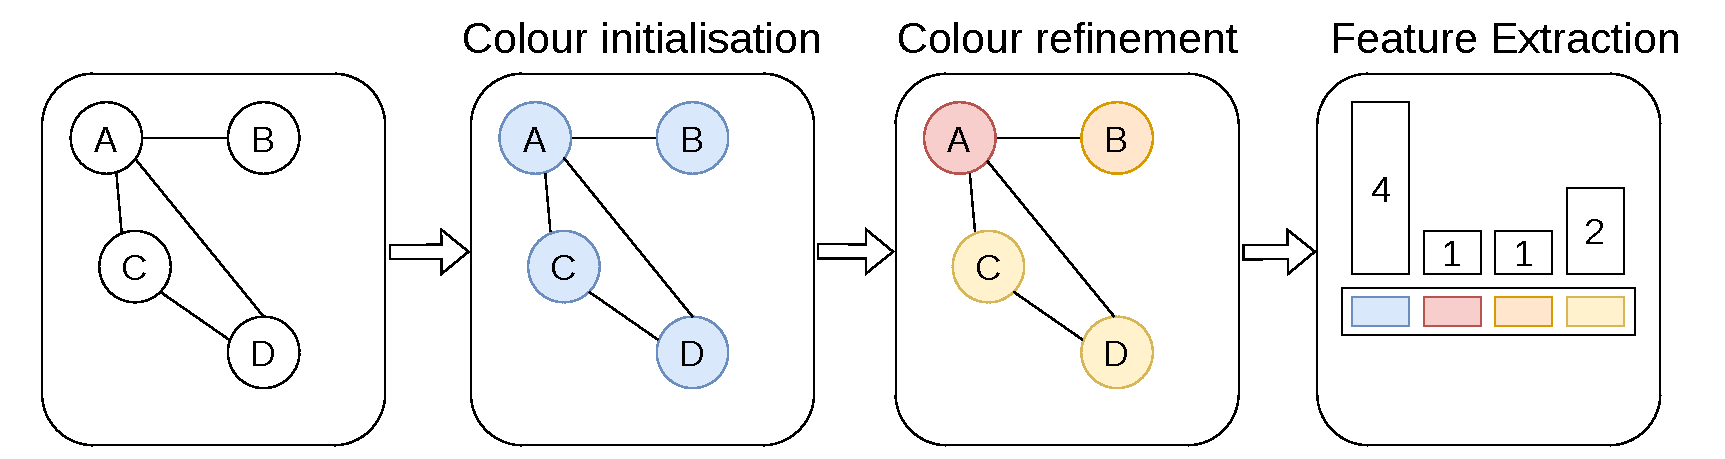
\includegraphics[width=.8\textwidth]{figures/wl.drawio.pdf}
    \caption{Feature extraction process using the WL algorithm on a simple, undirected graph. The colour refinement is executed only once. At first, all nodes get the same colour, then node A aggregates its colour (blue) with its 3 neighbours' colours (blue), getting, as a result, (blue, blue,blue,blue). This produces a new colour, red. C and D, having only two neighbours, get, as aggregation (blue, blue,blue), resulting in the new colour yellow and, finally, node B, having only one neighbour, aggregates to (blue, blue), getting as new colour orange. In the final steps, we count the number of occurrences of each colour, and we get 3 blues from the original initialisation and 1 red, 1 orange and 2 yellow after the first aggregation step.}
    \label{fig:wl-feature-exec}
\end{figure}

\subsection{WL For Feature Extraction}\label{sec:wl-feature_Extraction}
To use the WL algorithm for feature extraction, we repeat the colour refinement process for a pre-defined number of steps on a single graph, then we extract features by creating a histogram where, for each colour, we count the number of occurrences. Then, the final feature vector is created by concatenating the histograms after each iteration. A depiction of the execution of the WL algorithm for feature extraction (with one aggregation step) can be seen in Figure \ref{fig:wl-feature-exec}.

Note that while the standard WL feature extraction process typically concatenates histograms from all iterations, we deliberately utilise only the final histogram. This decision is informed by several theoretical and practical considerations specific to our domain.

First, from a theoretical perspective, the final iteration's labels represent the most refined partition of the graph's nodes. As demonstrated in the analysis of Graph Isomorphism Networks \cite{Xuetal2018}, the final state of a message-passing scheme (given an injective aggregation function) effectively encodes the full subtree structure. In our discrete WL implementation, the final labels serve as a compressed representation that implicitly preserves the structural history of previous iterations.

Furthermore, the specific topology of our data justifies this approach. The extracted graphs are characterised by a shallow diameter and directed edges, which significantly limit the depth of information flow. In such instances, the WL process converges rapidly as nodes quickly incorporate all available predecessors' information. Our empirical analysis (in Appendix \ref{sec:ablation-study}) across three distinct tasks and three different ML models confirmed this; we found no statistically significant difference in performance between concatenated features and the single-histogram approach. Consequently, we prioritise the latter.

\subsection{Enhancing Features' Expressiveness}
The standard WL features are designed for graphs without any edge or node information. However, in our case, we have both node and edge-level information we can use to better represent the input graph. For this reason, inspired by previous works \cite{Togninalli2019-qa},  we include two extensions to the base algorithm:
\begin{itemize}
    \item \textbf{Node-information extension}: To add node information into the extraction process, we can initialise the node colour with the hash of its type + subtype (e.g. a \texttt{Variable node} and a \texttt{Sum node} will be initialised with different colours). Formally, $c^{(0)}(v) \leftarrow \text{HASH}(\text{type}(v) \ || \ \text{subtype}(v))$ where $||$ denotes string concatenation.
    \item \textbf{Edge-information extension}: To add edge information into the extraction process, we can concatenate the edge type to the node colour during the aggregation step (e.g. in the example of Figure \ref{fig:wl-feature-exec}, if Node B was connected to node A via a Leading edge, the aggregation of node B would be: (blue, blue-L)). Formally, assuming a directed graph where edges flow towards $v$, its multiset update becomes $M(v) \leftarrow \{\!\!\{c^{(t-1)}(w) \ || \ \text{type}(w, v) \mid (w,v) \in E\}\!\!\}$.
\end{itemize}
Finally, we can use the fact that our graphs are directed and only update a node colour based on its incoming neighbours.

Using these extensions, we can now define four types of features: (i) \texttt{WL}, standard WL features without node or edge information, (ii) \texttt{WLn}, WL features enhanced via node-information extensions, (iii) \texttt{WLe},  WL features enhanced via edge-information extensions, and (iv) \texttt{WLne}, WL features enhanced with both edge and node-information. 

\subsection{The ``Cut'' Trick}
In the WL algorithm, the colour of a node is highly dependent on its degree, and two nodes with different degrees, even when sharing the same original colour and the same type of neighbour nodes, will end up with different colours. This can be problematic for nodes representing operators and constraints where the number of connected sub-elements can vary. As an example, let's examine the \texttt{all\_different} global constraint: using the standard algorithm, \texttt{all\_different([v1, v2, v3])} will get a totally different and uncorrelated colour to \texttt{all\_different([v1, v2])} solely due to its degree. In practice, while preserving some differences between the two constraints, we would still capture the fact that they are pretty similar.

To achieve this, we can virtually ``cut'' the connections between the nodes representing constraints and operators with a variable number of operands in them. We will refer to these nodes as cut nodes. In practice, during the aggregation steps, the cut nodes will not be updated since their incoming connections will be ignored. However, the cut nodes will still contribute to the update of the nodes they are connected to via their outgoing edges. All cut nodes can be seen in Appendix \ref{sec:node-types}. 

After the aggregation steps have been completed, each cut node's colour can be updated by aggregating it with the set (not multiset) comprised of all its connected, original node colours. By using a set rather than a multiset, nodes with the same type of incoming nodes will receive the same colour, independent of their degree.

At this stage, we can correctly capture the fact that two constraints with the same type of connected nodes but different degrees have the same colour; however, we are completely missing any information regarding the degree of a node, information that we would still like to capture. To do so, we can add extra features after the colour histogram. Specifically, from each cut node, we can generate node pairs comprising the cut node and its incoming neighbours. Thus, each cut of degree $n$ will generate $n$ pairs. After having generated all the pairs, we count the occurrence of each pair in a graph to generate a histogram of pairs and concatenate it to the histogram of colours.

The cut trick can only be applied when node information is present, thus, only to \texttt{WLn} and \texttt{WLne} features. We will call the features where the cut trick is applied \texttt{WLc-n} if only the cut is applied to \texttt{WLn} features and \texttt{WLc-ne} if the cut is applied to \texttt{WLne}. A formalisation of the \texttt{WLc-n} features can be seen in Algorithm \ref{alg:wl-cut}, and a graphical depiction of how the cut trick is applied can be seen in Figure \ref{fig:cut-trick}.

\begin{algorithm}[ht]
\scriptsize
\caption{\texttt{WLc-n} Algorithm for Feature Extraction. The \texttt{WLc-ne} version will be different only in the aggregation step, where the edge information will also be included.}
\label{alg:wl-cut}
\begin{algorithmic}[1]
\Require Graph $G = (V, E)$, iterations $T$, subset $V_{cut} \subseteq V$ of cut nodes
\Ensure Feature histograms of colours and pairs
\State \textbf{Initialisation:} $c^{(0)}(v) \leftarrow \text{HASH}(\text{type}(v) \,||\, \text{subtype}(v))$ for all $v \in V$
\State $t \leftarrow 0$
\Repeat
    \State $t \leftarrow t + 1$
    \For{each node $v \in V$}
        \If{$v \notin V_{cut}$}
            \State $M(v) \leftarrow \{\!\!\{c^{(t-1)}(w) \mid (w,v) \in E\}\!\!\}$
            \State $c^{(t)}(v) \leftarrow \text{HASH}(c^{(t-1)}(v), \text{sort}(M(v)))$
        \EndIf
    \EndFor
\Until{$t = T$}
\State $Pairs \leftarrow \{\!\!\{\}\!\!\}$ \Comment{Initialize multiset for pairs histogram}
\For{each node $v \in V_{cut}$}
    \State $S(v) \leftarrow \{ c^{(0)}(w) \mid (w,v) \in E \}$ \Comment{Set of initial colours (types) of incoming neighbours}
    \State $c^{(final)}(v) \leftarrow \text{HASH}(c^{(T)}(v), \text{sort}(S(v)))$
    \For{each node $w$ where $(w,v) \in E$}
        \State $Pairs \leftarrow Pairs \cup \{\!\!\{ (c^{(0)}(w), c^{(0)}(v)) \}\!\!\}$
    \EndFor
\EndFor
\State $c^{(final)}(v) \leftarrow c^{(T)}(v)$ for all $v \in V \setminus V_{cut}$
\State \Return $\text{Histogram}(c^{(final)}) \cup \text{Histogram}(Pairs)$
\end{algorithmic}
\end{algorithm}

\begin{figure}[t]
    \centering
    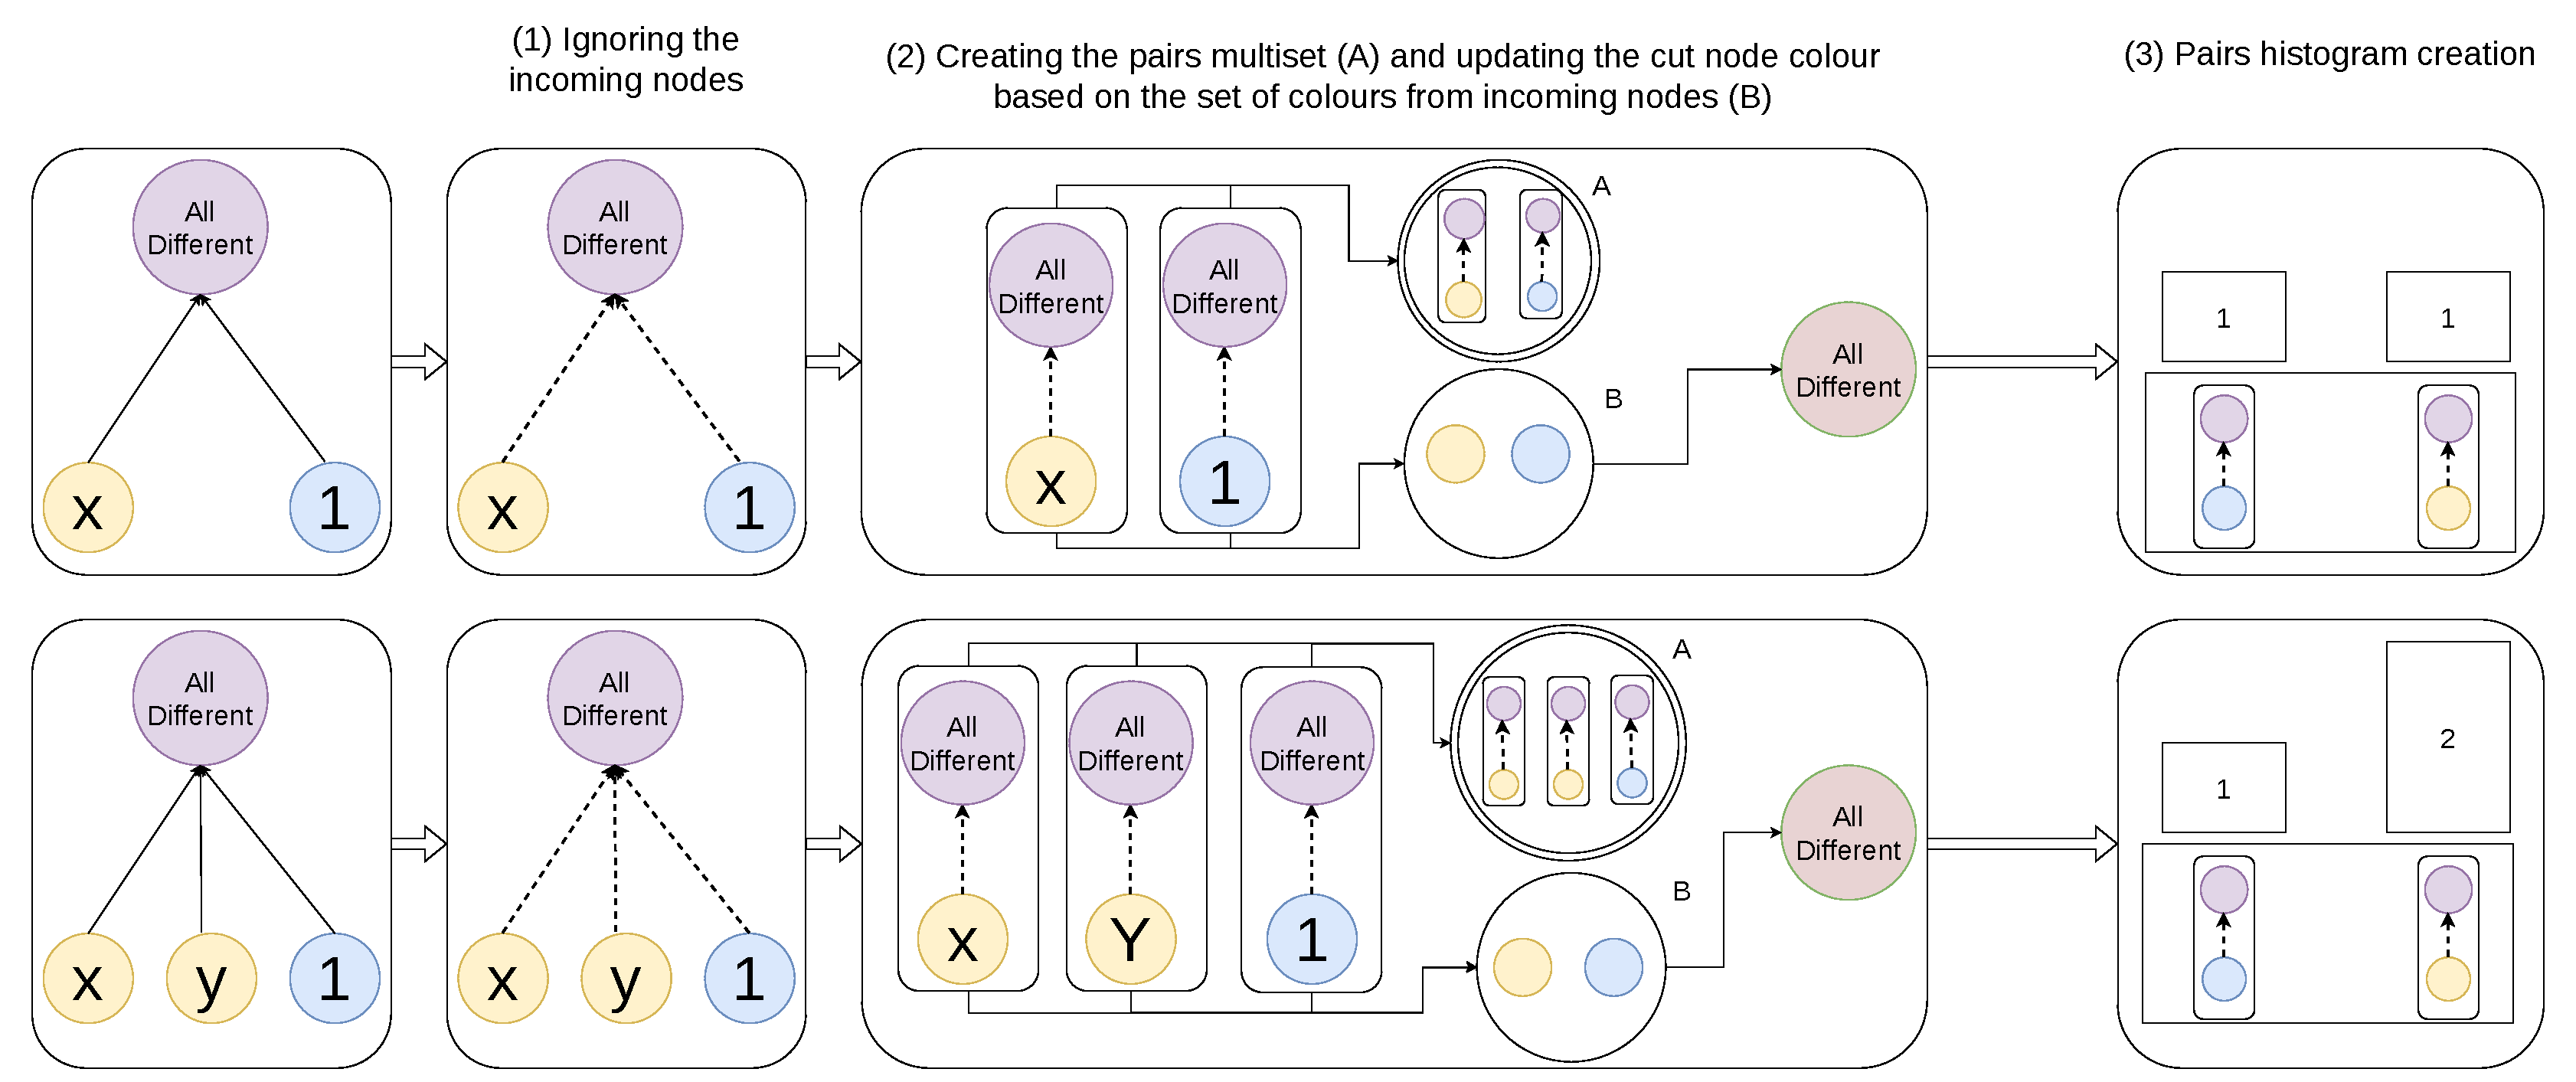
\includegraphics[width=.87\linewidth]{figures/wlc.drawio}
    \caption{Application of the cut trick on two occurrences of the \texttt{all\_different} constraint (top and bottom). Constraint nodes are in purple, variable nodes in yellow and parameter nodes in blue. First, cut nodes do not perform the normal WL aggregation steps (1), then we generate all pairs and update the colour of the \texttt{all\_different} node by aggregating it with the set of all types of node with incoming edges (2) and then we generate the pairs histogram by counting all the occurrences of the pairs (3). In this example, since both constraints share the same type of incoming nodes, they will be coloured in the same way. However, having a different node degree will result in a different pair histogram.}
    \label{fig:cut-trick}
\end{figure}

\subsection{Features, Characteristics, and Normalisation} \label{sec:feature_characteristics}
As a consequence of our design choices, especially of having directed graphs, the extracted features have emerging properties that are worth noting. In particular, since variable and parameter edges have no incoming node (but for the variable connected to the objective function), the colours of those values never get updated. Thus, one value in the final feature set would represent the number of variables in the graph, and another the number of parameters in the graph.

To give some extra information about variables and parameters in the graph, besides their total count, we decided to add two extra features, one representing the average number of constraints/operators a variable takes part in and one representing the same but for parameters.

Also, due to the direct nature of our graphs, most paths in the graph are quite shallow, especially after the cut. As an example, in the \texttt{x + 3 = y} constraint, we will have 2 variable nodes, (\texttt{x, y}), one parameter node (\texttt{3}), one operator node (\texttt{+}) and one constraint node (\texttt{=}). The operator node can be updated only once since the values of the parameter and variable nodes connected to it will never get updated. At the same time, the value of the constraint node can be updated at most twice: once at the first step when it aggregates with the original \texttt{+} and \texttt{y} colours and once at the second step when it aggregates with the updated \texttt{+} colour and the original, unmodified \texttt{y} colour. For a deeper discussion on the depth of the produced graphs, see Appendix \ref{sec:graph-depth}. 

Global constraints are always terminal nodes without any outgoing nodes; thus, as a consequence, updating them only once, at the end of the standard WL steps, will result in the same output as updating them during the standard WL steps.



Finally, once the final histograms are extracted from the graphs, we need to normalise the features. This is a necessary step since the values in the histograms will grow proportionally to the size of the graph. Thus, if not normalised, the produced histograms will be comparable only with those produced by graphs of the same size, making it impossible to generalise.

We decided to normalise the colour histograms by dividing each value in the histogram by the total count of nodes. Similarly, the pairs histogram is normalised by the total pairs count. This normalisation step will generate a final feature set with values always smaller than or equal to 1.

\subsection{Train and Test Feature Extraction Process}
During the extraction process, different graphs will generate different colours, and only a subset of those will be shared between different graphs. This will result in feature sets with different histogram sizes and with different colours in them. To train an ML model, we need to standardise the histograms, making them share the same colours. To do so, we can collect all colours from all histograms and add a 0 coefficient to all colours missing in a histogram. 

During testing, if we encounter a new colour not present in the training data, we simply discard it and ignore the update.